\documentclass[tikz,convert={outext=.svg,command=\unexpanded{pdf2svg \infile\space\outfile}},multi=false]{standalone}
\usepackage[utf8]{inputenc}

\usetikzlibrary{automata}% tikz package already loaded by 'tikz' option
\newcommand{\ascenseur}[5]{\begin{tikzpicture}[xscale=0.7]
\draw[draw=#5] (-0.3, 1.1) -- (-0.3, 1.5);
\draw[draw=#5] (-0, 1.1) -- (-0, 1.5);
\draw[draw=#5] (0.3, 1.1) -- (0.3, 1.5);
\draw[draw=#5] (-0.3, 0.9) -- (-0.3, 0.5);
\draw[draw=#5] (-0, 0.9) -- (-0, 0.5);
\draw[draw=#5] (0.3,0.9) -- (0.3,0.5);
\draw (-1, 2) -- (-1, 0) -- (1, 0) --(1, 2);
\draw[fill=#1, draw=none] (-0.8, 1) rectangle (0.8, 0);
\draw[fill=#2, draw=none] (-0.8, 2) rectangle (0.8, 1);
\draw[fill=#3] (1, 0.4) rectangle (1.2, 0.6);
\draw[fill=#4] (1, 1.4) rectangle (1.2, 1.6);
\end{tikzpicture}}
\begin{document}


\newcommand\xm5
\newcommand\xM{10}
\newcommand{\dessinmodele}{
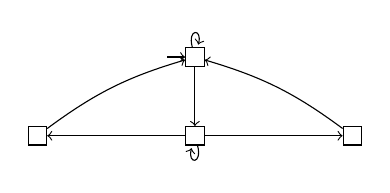
\begin{tikzpicture}[scale=0.5]
\tikzstyle{etat} = [draw, fill=white];
%\node (0bbm) {\ascenseur {black} {none} {white} {white} {white}};
%\node (0Bbm) at (\xm, 2) {\ascenseur {black} {none} {black} {white} {white}};
%\node (0BbM) at (\xM, 2) {\ascenseur {black} {none} {black} {white} {black}};
%\node (0bBm) at (\xm, -2) {\ascenseur  {black} {none}  {white} {black} {white}};
%\node (0bBM) at (\xM, -2) {\ascenseur {black} {none}  {white} {black} {black}};
%
%\node (0BBm) at (\xm, 0) {\ascenseur  {black} {none}  {black} {black} {white}};
%\node (0BBM) at (\xM, 0) {\ascenseur {black} {none}  {black} {black} {black}};
%
%\node (1bbm) at (0, 8) {\ascenseur {none} {black} {white} {white} {white}};
%\node (1Bbm) at (\xm, 10) {\ascenseur {none} {black} {black} {white} {white}};
%\node (1BbM) at (\xM, 10) {\ascenseur {none} {black} {black} {white} {black}};
%\node (1bBm) at (\xm, 6) {\ascenseur  {none} {black}  {white} {black} {white}};
%\node (1bBM) at (\xM, 6) {\ascenseur {none} {black}  {white} {black} {black}};
%
%\node (1BBm) at (\xm, 8) {\ascenseur   {none} {black}  {black} {black} {white}};
%\node (1BBM) at (\xM, 8) {\ascenseur  {none} {black}  {black} {black} {black}};
%
%\draw[->] (0bbm) edge (0Bbm);
%\draw[->] (0bbm) edge (0bBm);
%\draw[->] (0Bbm) edge (0BBm);
%\draw[->] (0bBm) edge (0BBm);
%
%\draw[->] (0bBm) edge (0bBM);
%\draw[->] (0bBm) edge (0bBM);
%\draw[->] (0BBm) edge (0BBM);
%
%\draw[->] (1bbm) edge (1Bbm);
%\draw[->] (1bbm) edge (1bBm);
%\draw[->] (1Bbm) edge (1BBm);
%\draw[->] (1bBm) edge (1BBm);
%
%\draw[->] (1Bbm) edge (1BbM);
%
%\draw[->] (0bBM) edge [bend right=10] (1bbm);
%\draw[->] (1BbM) edge [bend right=-10] (0bbm);
%\draw[->] (0BBM) edge  (1bBm);

\node[etat, initial left, initial text={}] (a) { };
\node[etat] (s)  at (0, -2) { };
\node[etat] (c1)  at (-4, -2) { };
\node[etat] (c2)  at (4, -2) { };
\draw[->] (a) edge[loop above] (a);
\draw[->] (s) edge[loop below] (s);
\draw[->] (a) -- (s);
\draw[->] (s) -- (c1);
\draw[->] (s) -- (c2);
\draw[->] (c1) edge[bend right=-10] (a);
\draw[->] (c2) edge[bend right=10] (a);
\end{tikzpicture}}



\newcommand\ok{%
\raisebox{-1mm}{%

\begin{tikzpicture}[scale=0.5]
\node [circle, fill=green!70!black, minimum height=5mm] at (0.3, -0.1) {};
\draw[line width=0.8mm, white] (0, 0) -- (0.2, -0.3) -- (0.6, 0.1);
\end{tikzpicture}}}
\newcommand\notok{%
\raisebox{-1mm}{%

\begin{tikzpicture}
\node [circle, fill=red!80!black, minimum height=5mm] at (0.1, 0.09) {};
\draw[line width=0.8mm, white] (0, 0) -- (0.2, 0.2);
\draw[line width=0.8mm, white] (0.2, 0) -- (0, 0.2);
\end{tikzpicture}}}


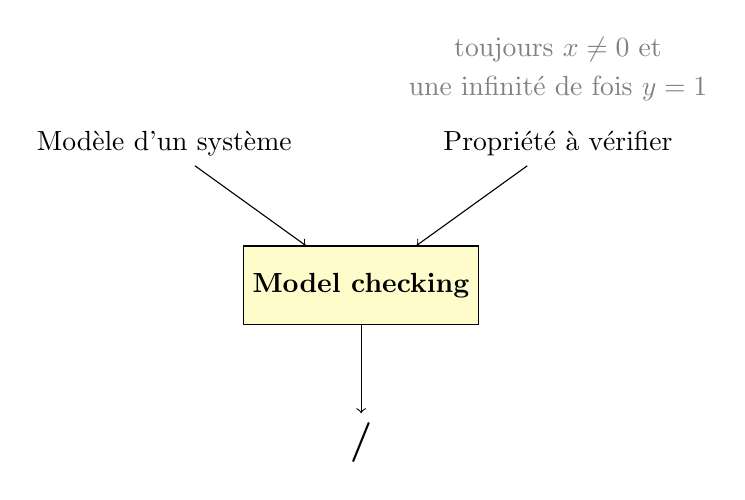
\begin{tikzpicture}
\node (m) at (0, -1.2) {Modèle d'un système };
\node[gray] { \dessinmodele};

\node[gray] at (5, 0) {toujours $x \neq 0$ et};
\node[gray] at (5, -0.5) {une infinité de fois $y = 1$};
\node (p) at (5, -1.2) {Propriété à vérifier};

\node[minimum height=1cm, draw, fill=yellow!20] (mc) at (2.5, -3) {\textbf{Model checking}};
\draw[->] (m) -- (mc);
\draw[->] (p) -- (mc);

\node [] (r) at (2.5, -5) {\ok {\Large{\textbf{/}}}\notok};
\draw[->] (mc) -- (r);

\end{tikzpicture}
\end{document}